
\chapter{Best Resources for Learning Synthesizable SystemVerilog}
\label{chapter:resources}

When writing synthesizable SystemVerilog, not all features present in the IEEE 1800 specification can be utilized, as synthesis tools support only a subset of these features. Unfortunately, many educational resources for Verilog and SystemVerilog fail to document which features are synthesizable and which are for verification only. To combat this ambiguity, a curated set of resources dedicated to synthesis should be prioritized when giving students additional materials for outside the classroom.

\section{Stuart Sutherland's synthesis guide is most valuable.}

``Synthesizing SystemVerilog: Busting the Myth that SystemVerilog is only for Verification'' by Stuart Sutherland and Don Mills acts as a comprehensive list of synthesizable SystemVerilog features. Despite the absence of an official SystemVerilog synthesis standard, this paper gives valuable insight into synthesizable language features, emphasizing their practical application into modern hardware designs. Sutherland and Mills surveyed the Synopsys tools Design Compiler and Synplify-Pro to trace the evolution of Verilog-1984 though SystemVerilog-2009 as a comprehensive hardware design and verification language. To assist those working on ``Labs with CVA6'', I composed a summary of Sutherland's synthesis guide \cite{labsWithCVA6}. Since then, I have shared this summary with dozens of students looking to improve their understanding of synthesizable Verilog. Providing both Sutherland's guide and my summary ensures that students receive a strong introduction to synthesizable Verilog syntax and best practices.

\section{Style guides record synthesizable features and best-practices.}

Even while avoiding unsynthesizable SystemVerilog features, design tools are infamous for misinterpreting syntax and often providing little or misleading information on errors. Therefore, following a well-verified style guide is crucial to ensure that an RTL implementation will work on an assortment of tools. As mentioned in \autoref{chapter:digital_design}, style guides help direct engineers away from ambiguous or poorly-supported language features, and towards styles and features that are verified to tape-out chips successfully. By introducing Verilog syntax alongside an exhaustive and highly-verified style guide, students can feel much more confident exploring new language features.

See [appx] for a(n incomplete) list of style guides. The lowRISC Style Guide discusses many best-practices surrounding language features such as the alias statement, automatic scopes, package imports, and floating begin-end blocks. The Bespoke Silicon Group Style Guide is also strong due to its discussion of structures, enumerations, and memories. Personally, I teach the lowRISC style guide because of the clarity in \mintinline{systemverilog}{_d} and \mintinline{systemverilog}{_q} as suffixes for register inputs and outputs, and to match the ``Labs with CVA6'' project. (See \autoref{chapter:labs_with_cva6}.)

\section{Verilog tutorial websites should be treated cautiously.}

It is important to stress the importance of following the provided style guides for Verilog syntax over some of the most popular Verilog tutorial websites, such as ASIC World, Chipverify, and Nandland. Despite the user-friendly approach adopted by these websites, which mirror renowned programming tutorial platforms such as GeekforGeeks, Verilog tutorial websites often propagate misguided advice for novice hardware developers. While style-guides can act as a reference to well-verified practices for beginners and professionals alike, tutorial websites do not always teach current-day, synthesizable design syntax that is compatible with a multitude of tools. Only if students maintain adherence to the instructor-specified style-guides and the subset of synthesizable features, then tutorial websites can be used as resources.


\begin{figure}[t]
    \centering
    \inputminted[frame=single]{systemverilog}{code/always_ff.svh}
    \caption{Potentially confusing behaviors of \mintinline{systemverilog}{always_ff} blocks}
    \label{fig:always_ff}
\end{figure}


\begin{figure}[t]
    \centering
    \frame{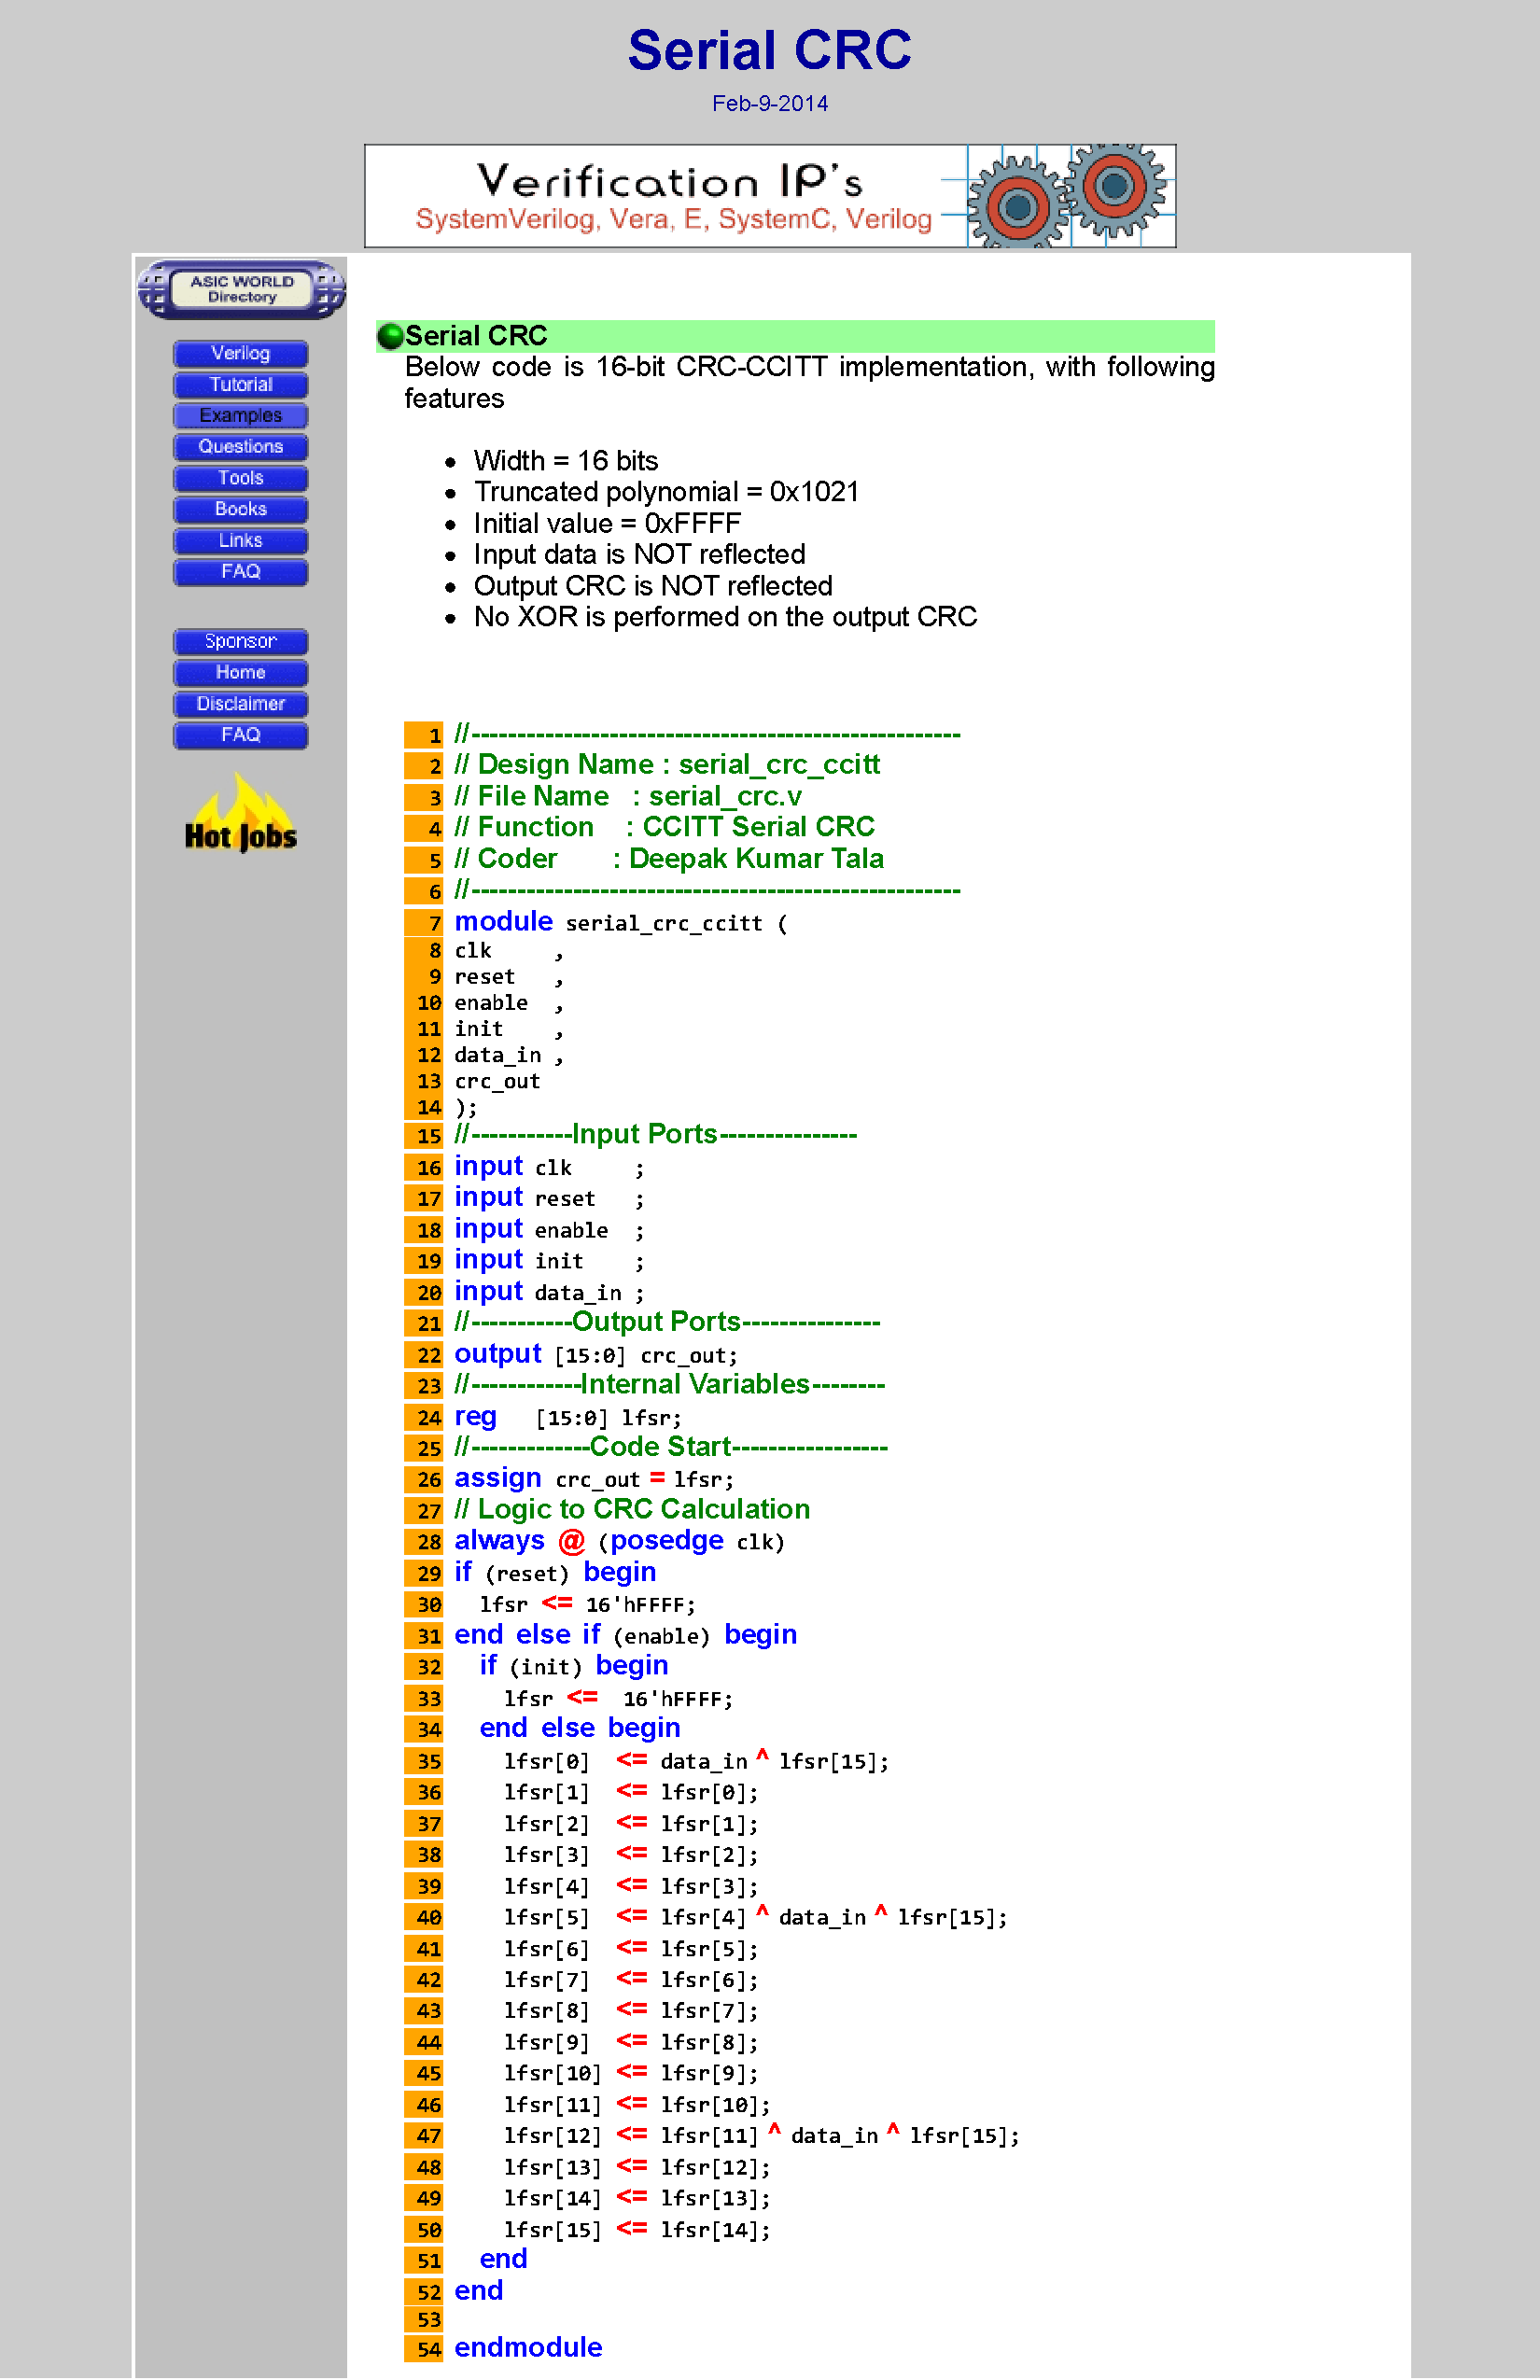
\includegraphics[width=\textwidth,height=0.9\textheight,keepaspectratio]{media/asicworld.pdf}}
    \caption{This is an example provided by ASIC World that encourages bad design practices \cite{asicworld}}
    \label{fig:asicworld}
\end{figure}


For example, while a TA for ECE 152A, 154A, and 154B, the most prevalent misinformation they encouraged in students was to put combinational logic inside of \mintinline{systemverilog}{always_ff} blocks. (See \autoref{fig:asicworld}). The lowRISC Style Guide, the BSG SystemVerilog Coding Standards, and the IEEE 1364.1-2005 Verilog Synthesis Standard all recommend only putting resets, sets, and enables in \mintinline{systemverilog}{always_ff} blocks \cite{lowRISCstyleguides, BSGstyleguide, 1364.1-2005}. Unnecessarily large \mintinline{systemverilog}{always_ff} blocks are prone to bugs because \mintinline{systemverilog}{always_ff} blocks don't offer warnings on unhandled code paths, blocking and nonblocking-assignment mismatches can lead to undefined behavior, and synthesis tools may incorrectly infer the incorrect type of flip-flop. (See \autoref{fig:always_ff}) In my experience teaching SystemVerilog, whenever a student asked for help solving a bug, but followed this design practice, I immediately asked them to separate the block into an \mintinline{systemverilog}{always_comb} and \mintinline{systemverilog}{always_ff}. Over half the time, that simple refactor incidentally fixed the student's bug.

\FloatBarrier

\section{ChipDev.io can be used to practice Verilog (if used effectively).}


\begin{figure}[t]
    \centering
    \frame{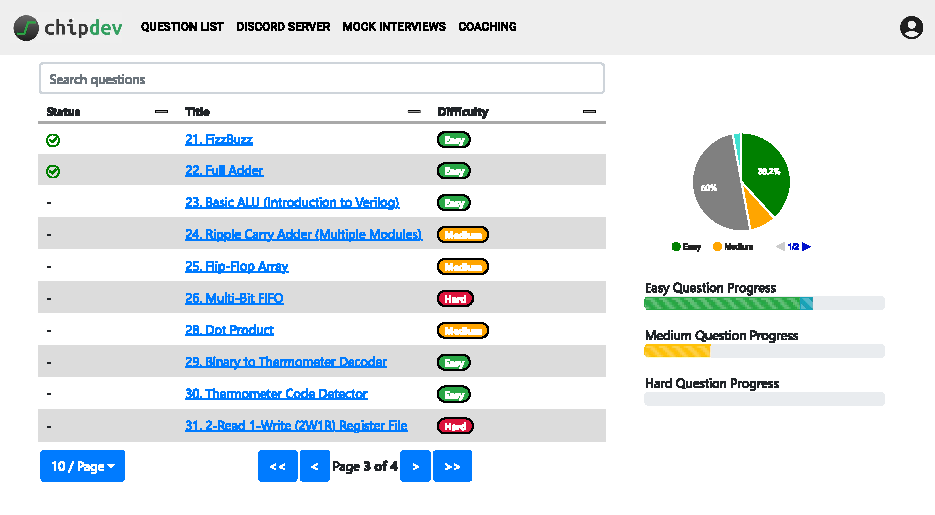
\includegraphics[width=0.7\linewidth]{media/chipdev_questions.pdf}}
    \caption{An example of questions that ChipDev offers. \cite{ChipDev}}
    \label{fig:chipdev_questions}
\end{figure}


\begin{figure}[t]
    \centering
    \frame{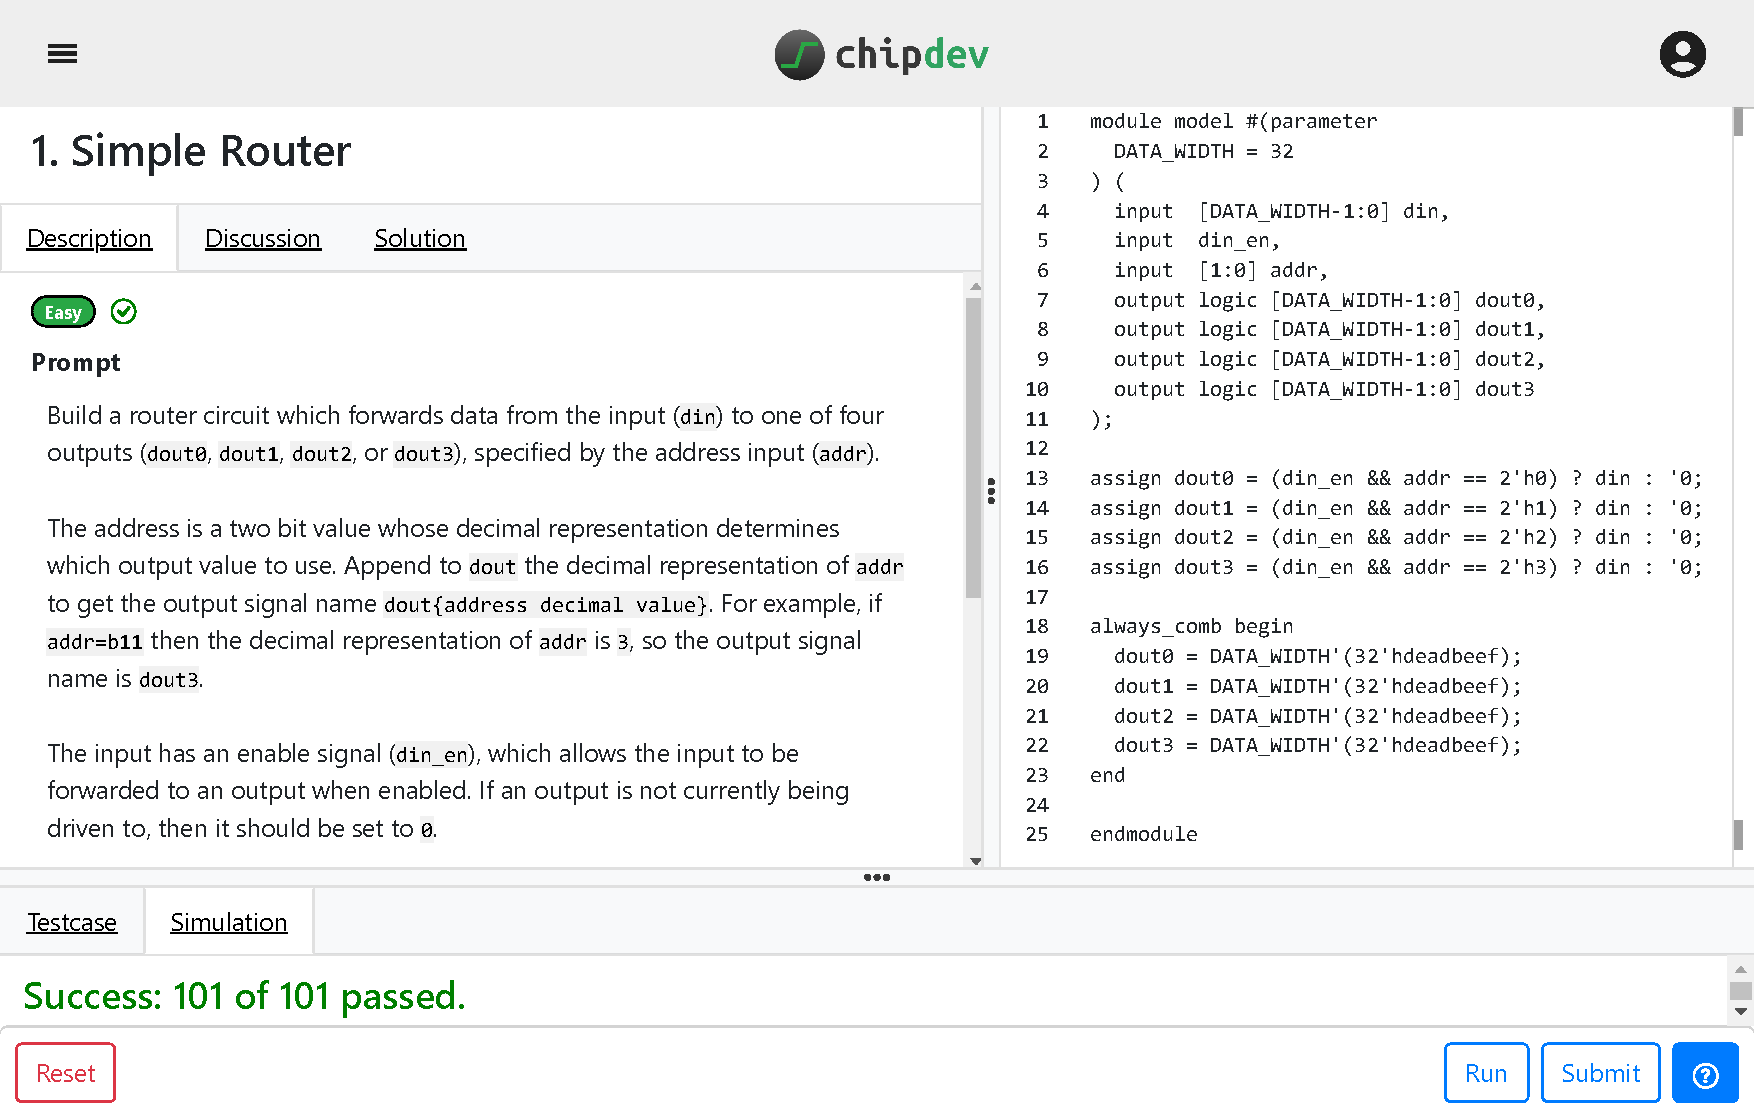
\includegraphics[width=0.9\linewidth]{figures/chipdev_hack.pdf}}
    \caption{This example shows ChipDev \cite{ChipDev} incorrectly accepting this submission despite a potential mismatch between simulation and synthesis. For example, Verilator will override the \mintinline{systemverilog}{always_comb} with the \mintinline{systemverilog}{assign}, but Yosys will override the \mintinline{systemverilog}{assign} with the \mintinline{systemverilog}{always_comb}. This could be corrected if ChipDev chooses to incorporate a similar verification flow to what is outlined in \autoref{section:complex_tool_setups}.}
    \label{fig:chipdev_hack}
\end{figure}


The final resource I like to share with students is ChipDev.io, which offers an online collection of popular Verilog questions, paired with an online IDE and testbench. The 30+ questions range from implementing a shift register to designing an ALU; (see \autoref{fig:chipdev_questions}.) If students are looking for lots of practice questions as job interview preparation or for general practice, I always recommend ChipDev. However, ChipDev does not run gate-level simulation or logical equivalence checks, so bad submissions may be incorrectly rewarded; (see \autoref{fig:chipdev_hack}.) Plus, after speaking with the ChipDev team, they notified me that synthesis was not on their priority list. Therefore, I strongly urge students to verify their answers with DigitalJS Online or other synthesis tools before feeling they have a mastery over any question.
